%
% $RCSfile: data_transfer_object.tex,v $
%
% Copyright (c) 2001-2004. Christian Heller. All rights reserved.
%
% No copying, altering, distribution or any other actions concerning this
% document, except after explicit permission by the author!
% At some later point in time, this document is planned to be put under
% the GNU FDL license. For now, _everything_ is _restricted_ by the author.
%
% http://www.cybop.net
% - Cybernetics Oriented Programming -
%
% http://www.resmedicinae.org
% - Information in Medicine -
%
% @author Christian Heller <christian.heller@tuxtax.de>
%

\subsection{Data Transfer Object}
\label{data_transfer_object_heading}

It is a well-known fact that many small requests between two processes, and even
more between two hosts in a network need a lot of time. The local machine with
two processes has to permanently exchange the program context and the network
has a lot of transfers. For each request, there is at least a necessity of two
transfers -- the question of the client and the answer of the server.\\
Transfer-methods are often expected to deliver common data such as a Person's
address, i.e. surname, first name, street, zip-code, town etc. These information
is best retrieved by only one transfer-call. That way, the client has to wait
only once for a server response and the server does not get too many single
tasks. In the address-example, all address data would best be packaged together
and sent back to the client.

\begin{figure}[ht]
    \begin{center}
       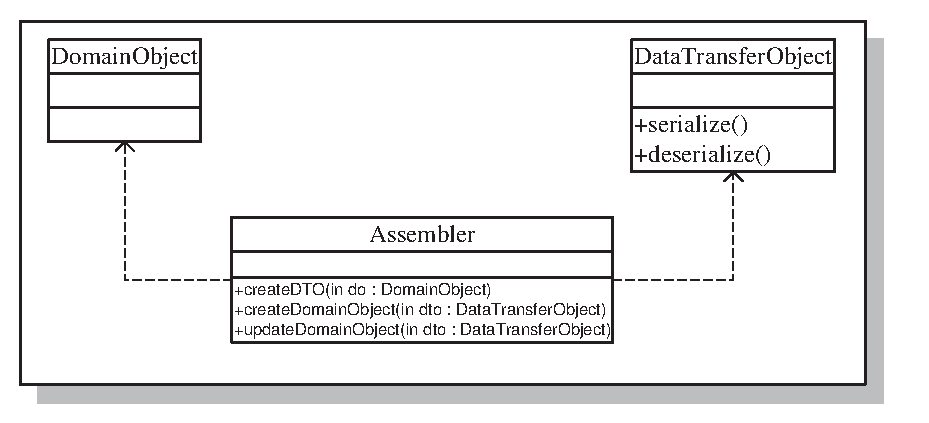
\includegraphics[scale=0.5]{vector/data_transfer_object.eps}
       \caption{Data Transfer Object Design Pattern \cite{fowler2002}}
       \label{data_transfer_object_figure}
    \end{center}
\end{figure}

And that is exactly what the Data Transfer Object pattern (figure
\ref{data_transfer_object_figure}) proposes a solution for: A central
\emph{Assembler} class takes all common data of the server's domain model object
and assembles them together into a special object called \emph{Data Transfer Object}
(DTO) which is a flat data structure.
The server will then send this DTO over network to the client. On the client's side,
a similar assembler takes the DTO, finds out all received data and maps (disassembles)
them to the client's domain model. In that manner, a DTO is able to drastically
improve the performance in communications.\\
Comparing with the Data Mapper from chapter \ref{data_mapper_heading}, the
assembler's task of translating between data models seems quite similar, if not
the same. Hence, why shouldn't it be possible for inter-system communications
over network to use a \emph{Translator} similar to the one for persistence?
This translator could provide special parts for assembling different types of
DTOs, independent from which communication protocol/language (Sockets, RMI, JMS,
CORBA, SOAP etc.) is used.

